%%%%%%%%%%%%%%%%%%%%%%%%%%%%%%%%%%%%%%%%%%%%%%%%%%%%%%%%%%%%%%%%%%%%%%
% How to use writeLaTeX:
%
% You edit the source code here on the left, and the preview on the
% right shows you the result within a few seconds.
%
% Bookmark this page and share the URL with your co-authors. They can
% edit at the same time!
%
% You can upload figures, bibliographies, custom classes and
% styles using the files menu.
%
% If you're new to LaTeX, the wikibook is a great place to start:
% http://en.wikibooks.org/wiki/LaTeX
%
%%%%%%%%%%%%%%%%%%%%%%%%%%%%%%%%%%%%%%%%%%%%%%%%%%%%%%%%%%%%%%%%%%%%%%
\documentclass{tufte-handout}

%\geometry{showframe}% for debugging purposes -- displays the margins

\usepackage{amsmath}

% Set up the images/graphics package
\usepackage{graphicx}
\setkeys{Gin}{width=\linewidth,totalheight=\textheight,keepaspectratio}
\graphicspath{{graphics/}}

\title{Hands-On Session: Data Encryption}
\author{DIME Analytics \\ \href{mailto:dimeanalytics@worldbank.org}{dimeanalytics@worldbank.org}}
\date{12 June 2019}  % if the \date{} command is left out, the current date will be used

% The following package makes prettier tables.  We're all about the bling!
\usepackage{booktabs}

% The units package provides nice, non-stacked fractions and better spacing
% for units.
\usepackage{units}

% The fancyvrb package lets us customize the formatting of verbatim
% environments.  We use a slightly smaller font.
\usepackage{upquote}
\usepackage{fancyvrb}
\fvset{fontsize=\normalsize}
\renewcommand{\FancyVerbFormatLine}{\color{violet}}
\DefineShortVerb{\|}

% Small sections of multiple columns
\usepackage{multicol}

% Provides paragraphs of dummy text
\usepackage{lipsum}

 \usepackage{float}

% These commands are used to pretty-print LaTeX commands
\newcommand{\doccmd}[1]{\texttt{\textbackslash#1}}% command name -- adds backslash automatically
\newcommand{\docopt}[1]{\ensuremath{\langle}\textrm{\textit{#1}}\ensuremath{\rangle}}% optional command argument
\newcommand{\docarg}[1]{\textrm{\textit{#1}}}% (required) command argument
\newenvironment{docspec}{\begin{quote}\noindent}{\end{quote}}% command specification environment
\newcommand{\docenv}[1]{\textsf{#1}}% environment name
\newcommand{\docpkg}[1]{\texttt{#1}}% package name
\newcommand{\doccls}[1]{\texttt{#1}}% document class name
\newcommand{\docclsopt}[1]{\texttt{#1}}% document class option name

\begin{document}

\maketitle% this prints the handout title, author, and date

\begin{marginfigure}%
  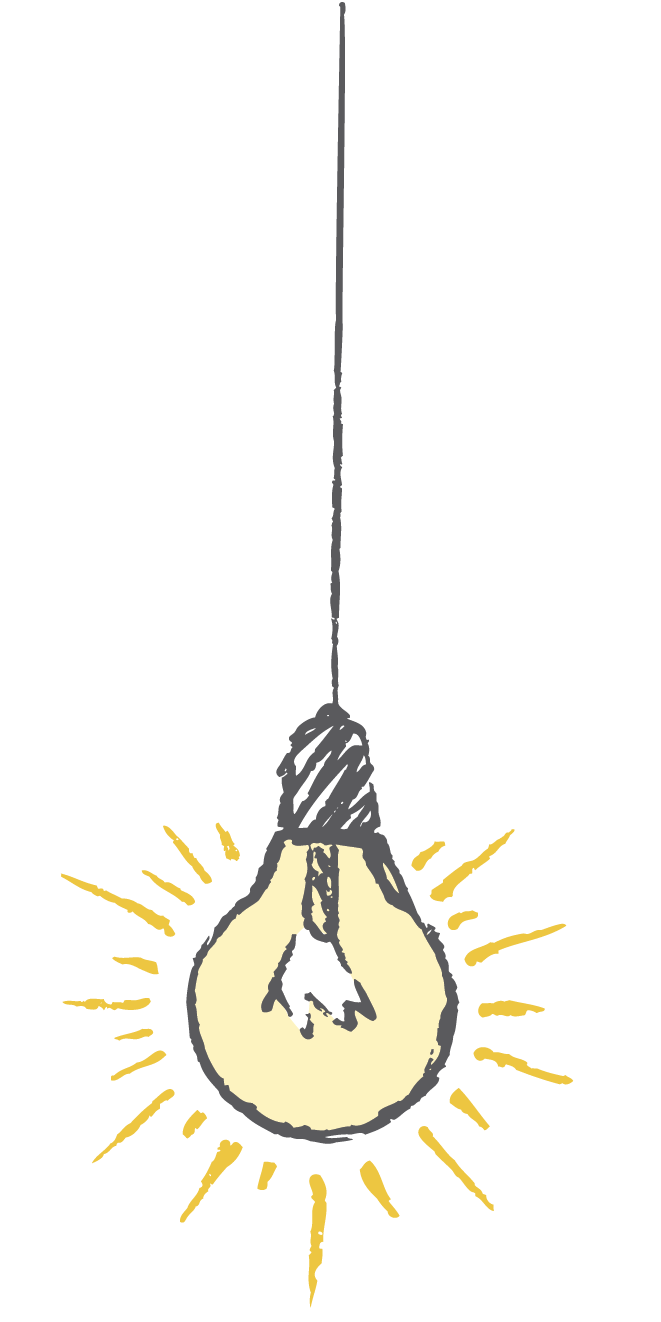
\includegraphics[width=\linewidth]{img/light.png}
\end{marginfigure}

\begin{abstract}
In this exercise we will encrypt a dataset and attempt to access the data in an encrypted folder

\bigskip\noindent \textbf{Exercise Objectives}: On completing this exercise you will be able to
\begin{enumerate}
  \item Download and install VeraCrypt
  \item Set up a secure folder using VeraCrypt
  \item Encrypt files in the secure folder
  \item Access the encrypted files in the secure folder
\end{enumerate}
\end{abstract}

%\printclassoptions
\section{Part 1: Download and install VeraCrypt}

VeraCrypt is the software that we recommend for use when encrypting data on your computer, regardless if it is an a non-shared folder, or a shared folder like DropBox. VeraCrypt is a free open-source software so you can use it without having to pay for it.

The first time we use VeraCrypt we need to download and install the software. If you are using a World Bank desktop, then you must make an \textit{eServices} request and have an IT person installing the software for you.

If you are not using World Bank computer, then you can download the software here: \url{https://www.veracrypt.fr/en/Downloads.html}. For Mac computers there is the installer version, choose that one. For Windows users there are 4 version, choose the \textit{installer}-version. After you have downloaded the installer file, open it and follow the instructions. Most people do not need to change any of the default values.

Anyone in your team that want to access the files you encrypt with VeraCrypt will also have to download the software to be able to access the files.

\section{Part 2: Set up VeraCrypt}

Before you can encrypt any files on your computer you must use VeraCrypt to create a special folder. In VeraCrypt this is called a \textit{Volume} but think of this as a very secure folder that you access in a different way.

\begin{enumerate}

	\item If you have VeraCrypt open, start by closing it, and re-open it. All our instructions will start from the opening page.
	\item On the opening page click \textit{Create Volume} (marked in read in the image below). Remember that \textit{Volume} in VeraCrypt means secure folder.


	\begin{figure}%
		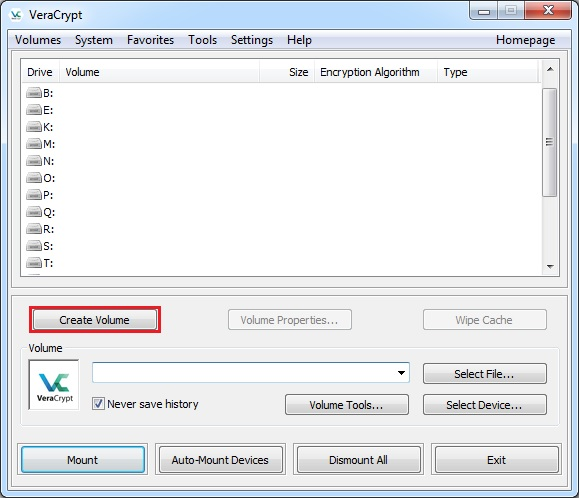
\includegraphics[width=.9\linewidth]{img/vc_install_1.png}
	\end{figure}
	\FloatBarrier
		
	\item In \textit{The VeraCrypt Volume Creation Wizard} you have three options. VeraCrypt has many very advanced options, but for the type of work we do we will only use the simplest option which is creating \textit{encrypted file container} type of volumes which is the default option.
	
	\begin{figure}
		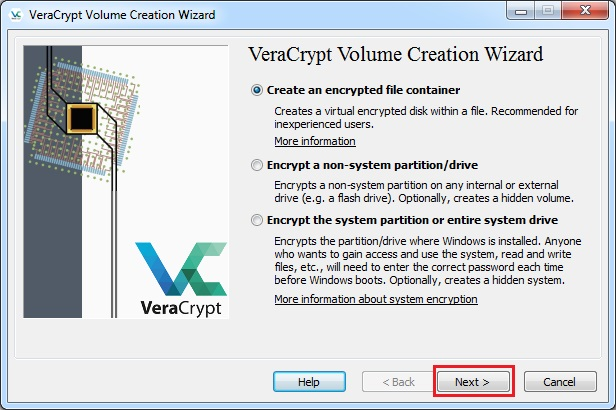
\includegraphics[width=.9\linewidth]{img/vc_install_2.png}
	\end{figure}
	\FloatBarrier
	
	\newpage
	
	\item In the next step, we will again choose the simplest options and create a \textit{Standard VeraCrypt volume} and then click \textit{Next}.
	\begin{figure}
		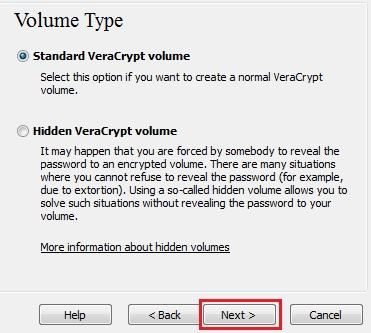
\includegraphics[width=.75\linewidth]{img/vc_install_3.png}
	\end{figure}
	\FloatBarrier
	
	\item Next you have to specify where you want to create the secure folder \textit{volume}. The volume behaves as a folder where you can store files, but technically it is a file (you do not need to understand how it works). So choose a location and give the volume file a name. Click select file. \sidenote{Note that a VeraCrypt container is just like any normal file. It can be, for example, moved or deleted as any normal file.}
	\begin{figure}%
		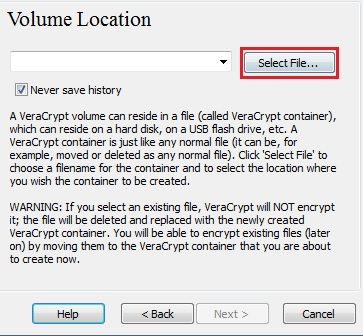
\includegraphics[width=.75\linewidth]{img/vc_install_4.png}
	\end{figure} 
	\FloatBarrier
	
	\newpage
	
	\item Select the desired path in the file selector. If you intend to share this folder, for example through DropBox, then this should be inside your DropBox folder. If you are using DIME Analytics' folder set-up then you should create this inside the encrypted folder.\sidenote{\url{https://dimewiki.worldbank.org/wiki/DataWork_Folder\#Survey_Encrypted_Data}}. Then type the name of the secure folder in the \textit{file name} box (remember the secure folder volume is actually a file). The rest of these examples assumes you call the file \textit{EncryptedData}. Then click \textit{Save}.
	
	\begin{figure}%
		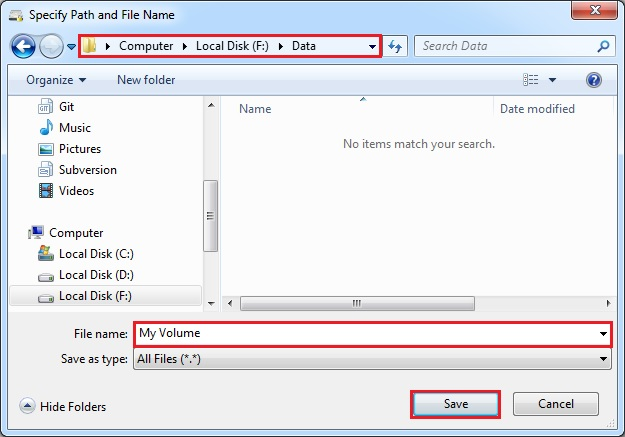
\includegraphics[width=.8\linewidth]{img/vc_install_5.png}
	\end{figure}
	\FloatBarrier
	
	
	\item Back in the \textit{Volume Creation Wizard} window, click \textit{Next}.
	\begin{figure}%
		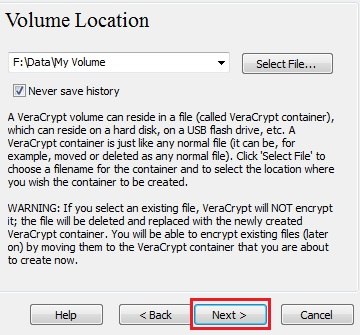
\includegraphics[width=.8\linewidth]{img/vc_install_6.png}
	\end{figure}
	\FloatBarrier
	
	\newpage
	
	\item One of the restrictions of VeraCrypt is that you already at this stage need to decide what the maximum size of the secure folder will be. Do not exaggerate too much, as the secure folder will always take up this much disk space, even when it is empty.\sidenote{If you end up choosing too small volume size, you can in the future create a new larger volume and move the files there.} In this example, choose 250 megabyte and then click \textit{Next}.
	\begin{figure}%
		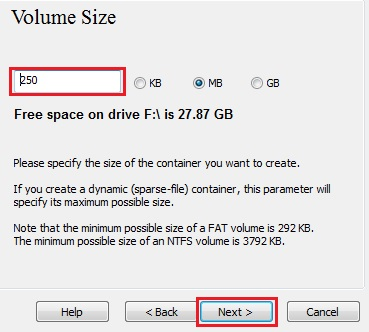
\includegraphics[width=.7\linewidth]{img/vc_install_7.png}
	\end{figure}
	\FloatBarrier
	
	
	\item In the next step you need to create a secure password.\sidenote{We recommend using a password manager like LastPass \url{https://www.lastpass.com/password-generator} to create a secure password. Lastpass \url{https://www.lastpass.com/} also be used to store and share passwords, especially complicated and long passwords required by softwares like VeraCrypt. If you are working in a World Bank project you can get access to LastPass \href{https://worldbankgroup.sharepoint.com/sites/ITS/cybersecurity-blog/Pages/Last-Pass-03062019-161721.aspx?deliveryName=DM10667}{Premium version} for free, but the basic version that is free for everyone will suit all your needs for this purpose.} Read VeraCrypt's instructions for what is a good password. After you have chosen your password, type it in the first input field and then re-type it in the second input field, and then click \textit{Next}.
	\begin{figure}%
		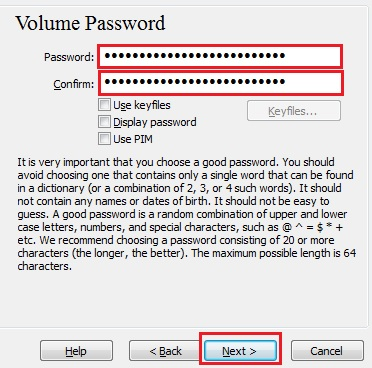
\includegraphics[width=.7\linewidth]{img/vc_install_8.png}
	\end{figure}
	\FloatBarrier
	
	
	\item To make the encryption completely unpredictable, VeraCrypt use your mouse movement to get a random input. Move your mouse inside the VeraCrypt window until the randomness indicator becomes green. The longer you move the mouse, the better. Then click \textit{Format}.
	\begin{figure}%
		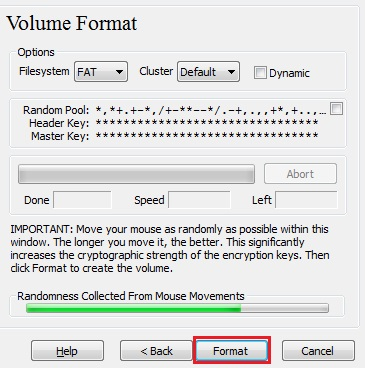
\includegraphics[width=.7\linewidth]{img/vc_install_9.png}
	\end{figure}
	\FloatBarrier
\end{enumerate}

	\noindent You have now created the secure folder. Go to the location where you created the folder to confirm it exists. It does not look like a folder, as it is technically a file. Double click on the folder to try and open it directly. Confirm that it doesn't open and you cannot do anything with it. Also see that the file is about 250MB big (or whatever value you chose) despite being still empty. Next part shows you how to use the secure folder.

%\printclassoptions
\section{Part 3: Add files to your secure folder}

	In this part, we will learn how to use VeraCrypt to make the secure folder appear like a folder and not like a file. This is called \textit{mounting} the volume. After you have mounted the volume you can add files to it just the same way that you add files to a regular folder.
	
	You need to re-mount the secure folder each time you start the computer and this is an important feature that makes your secure folder secure. Since you should not keep all your data files in the secure folder, only the data files with identifying or otherwise sensitive data, so the process of mounting and re-mounting the secure folder should not be too burdensome.
	
	Two important notes on encrypting files with VeraCrypt:
	
	i. VeraCrypt will not modify your files, it is more as if it puts a layer over your file, so that no-one can see the content or even what type of file it is or how big it is. Once this layer is removed (see next part of this exercise), the file and the content of it will be exactly the same as before you encrypted it.
	
	ii. After you have copied your files to the encrypted volume you created using VeraCrypt you must make sure that the files are deleted in their original location, because VeraCrypt does not encrypt any files still stored at the original location.
	

\begin{enumerate}
	\item If you have VeraCrypt open, start by closing it, and re-open it. All our instructions will start from the opening page.
	
	\item First you need to select a drive that will be used when you mount your secure folder. Even though the file you created in the last part might be stored on the \textit{C:} you need to select a different drive when mounting it. You can select any drive, but the examples in the rest of this exercise assumes that you select \textit{M:} as your drive.
	\begin{figure}%
		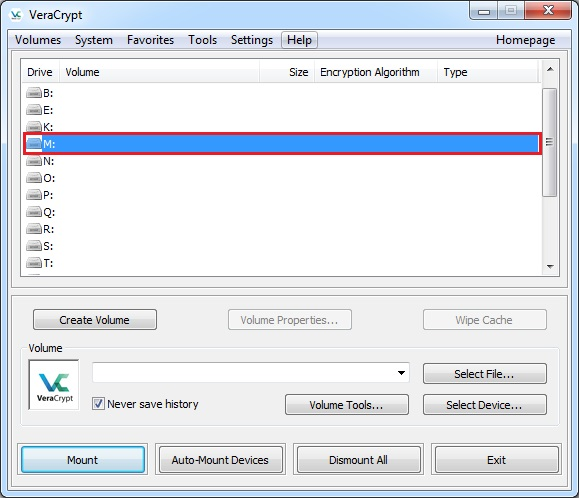
\includegraphics[width=.8\linewidth]{img/vc_mount_1.png}
	\end{figure}
	\FloatBarrier
	
	\item Then click \textit{Select File}.
	\begin{figure}%
		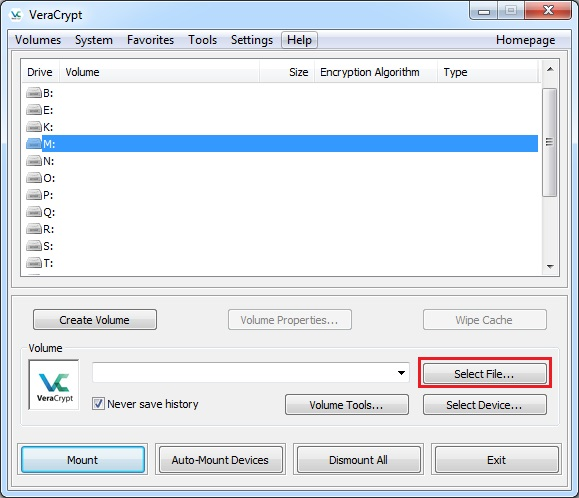
\includegraphics[width=.8\linewidth]{img/vc_mount_2.png}
	\end{figure}
	\FloatBarrier	
	
	\item In the file selector, browse to the volume file that we created in the last part and select it. Then click \textit{Open}.
	\begin{figure}%
		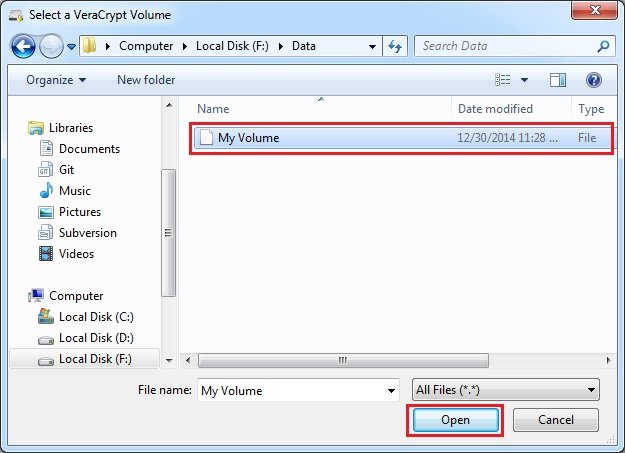
\includegraphics[width=.85\linewidth]{img/vc_mount_3.png}
	\end{figure}
	\FloatBarrier
	

	\item Back in the opening VeraCrypt window, click \textit{Mount}.
	\begin{figure}%
		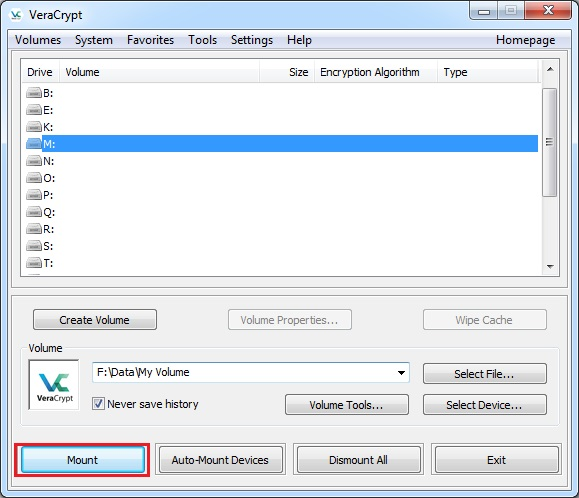
\includegraphics[width=.85\linewidth]{img/vc_mount_4.png}
	\end{figure}
	\FloatBarrier
	
	\newpage
	
	\item Type the password you created when you created the secure folder then click \textit{OK}.
	\begin{figure}%
		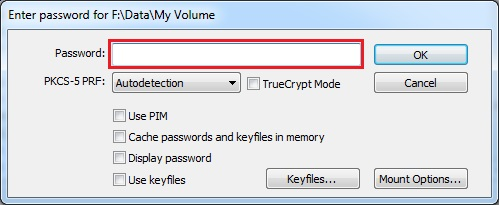
\includegraphics[width=\linewidth]{img/vc_mount_5.png}
	\end{figure}
	\FloatBarrier
	
	\item If the password is correct, we will have successfully mounted on the container as a virtual disk \textit{M:}. Double click on the disk \textit{M:} to open the container. 
	\begin{figure}%
		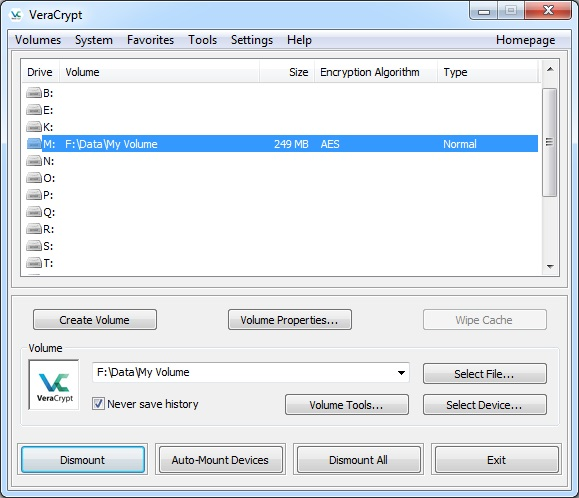
\includegraphics[width=\linewidth]{img/vc_mount_6.png}
	\end{figure}
	\FloatBarrier
	
	\item This will now open an empty folder in your file explorer. This empty folder has the file path \textit{M:}. This is very similar to when you plug in a USB/flash drive to your computer. 
	
	\item Save some files in the empty folder. This could be any type of files even though we will most often store data files in this folder. If you have access to the data sets used in DIME Analytics' \textit{Manage Successful Impact Evaluation Workshop}'s test files, then copy of the data sets titled \texttt{endline\_data\_raw.dta} and \texttt{panel\_data.dta} to the folder.
	
	\item You have now stored the files you added to the secure drive. However, as long as you have the secure folder mounted it can freely be accessed on \textit{M:} drive by anyone who has access to your computer. So go back to VeraCrypt, make sure that the mounted drive is highlighted and then click \textit{Dismount}. Once you do that, then there is no way to access these files without the password you used when creating the secure folder volume, even if someone gets access to your computer or your hard drive.
	
	
\end{enumerate}


%\printclassoptions
\section{Part 4: Access encrypted files}

In this part we will learn how to access the files in the secure folder. This is very similar to how we added files to the secure folder.

\begin{enumerate}
	\item If you have VeraCrypt open, start by closing it, and re-open it. All our instructions will start from the opening page.
	\item Mount the encrypted volume you created onto drive \textit{M:} but you can select any drive any time you mount the drive. However, as you will see soon it will be easier for you when you access the files in, for example, Stata if you are using the same drive for the same folder each time.
	\item Double click the mounted volume in the VeraCrypt window and see that the folder contains the folder you encrypted in the last part. If you were to access one of these files in Stata then you would use the file path \texttt{M:/endline\_data\_raw.dta} (if \textit{M:} was the drive that you chose). Not that even though you created the secure folder volume file somewhere on the \textit{C:} drive, the only way Stata can read it is through the mounted drive \textit{M:} (or whichever drive you chose).
	\item Once you are done working with the file containing identifying data that you keep in your secure folder, always make sure to directly unmount it in VeraCrypt.   
\end{enumerate}

\newpage

\section{Part 5: Pair up and share a secure folder with someone else (If time permits)}
Pair up with another person in the room and try to create, share, and access encrypted data.
\begin{enumerate}
	\item Create a shared Dropbox/Box/Onedrive folder.
	\item Create one secure  folder each in this shared folder. Use a simple password this time you do not mind sharing with the person you paired up with, but do not share the password yet.
	\item Look at your own and each other's file on the shared drive.
	\item Mount the secure folder in your computer and place some files in your secure folder in the shared Dropbox/Box/Onedrive folder.
	\item While you both have your own secure folder mounted, does the file look different when you look at it in the shared folder? Can you tell if files were added or not? Can you tell if someone else has the file mounted?
	\item Now share the password with your partner. How do you securely share a password?
	\item Access your partner's encrypted file by mounting it on VeraCrypt using the password your partner shared with you.
\end{enumerate}

\end{document}
